\documentclass{szzclass}
\usepackage{dependencies/szz-code}
\setminted{mathescape, escapeinside=||}

\subject{PPA}
\code{BI-WSI-SI-15}
\topic{Funkcionální programování, funkce vyšších řádů, Lisp: atomy, seznamy, funkce, cons buňky, rekurze, mapovací funkcionály.}

\begin{document}

\tableofcontents
\newpage

\section{Funkcionální programování}
\begin{itemize}
\item Zaměřeno na funkce a jejich vyhodnocování.
\item Nemá přiřazovací příkaz, nemá vedlejší efekty, typické používání rekurze.
\item LISP, Haskell, R, Clojure, Python
\item Odpovídající základní model výpočtu lambda kalkulus.
\item Má funkce vyšších řádů: parametrem i výsledkem funkce může být funkce. Má typicky uzávěry (closures).
\end{itemize}

\section{Lisp}
\begin{itemize}
\item Jeden z funkcionálních programovacích jazyků.
\item První jazyk, co měl garbage collection.
\item Lisp je case insensitive.
\end{itemize}

Lisp vyhodnocuje nejdřív argumenty (podvýrazy) a potom to zbytek, pokud mu to nezakážeme příkazem \mintinline{lisp}{quote} (zkratka apostrof):
\begin{minted}{lisp}
'(+ 1 1) |$\Leftrightarrow$| (quote (+ 1 1))| je ve výsledku |(+ 1 1)
\end{minted}

\begin{figure}[H]
  \centering
  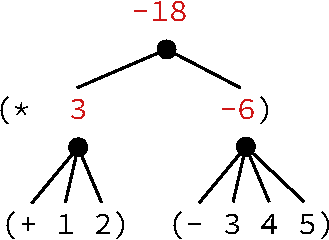
\includegraphics[width=4.2cm]{topics/bi-wsi-si-15/images/eval-tree}
  \caption{Vyhodnocení výrazu \mintinline{lisp}{(* (+ 1 2) (- 3 4 5))}}
\end{figure}

\subsection{Atomy}
  \begin{description}
    \item [čísla] \mintinline{lisp}{235.4 2e10 2/3}
    \item [proměnné] \mintinline{lisp}{foo 2nd-place *foo*}
    \item [konstanty] \mintinline{lisp}{pi t nil}
    \item [řetězce, znaky] \mintinline{lisp}{"Hello!" #\a}
    \item [pole] \mintinline{lisp}{#(1 "foo" A) #1A(1 "foo" A) #2A((A B C) (1 2 3))}
    \item [struktury] \mintinline{lisp}{#s(place FIT Prague)}
    \item [bitová pole] \mintinline{lisp}{#*10110}
    \item [hašovací tabulky]
  \end{description}

\subsection{Seznamy}
\begin{figure}[H]
\centering
\begin{minipage}{.5\textwidth}
  \centering
  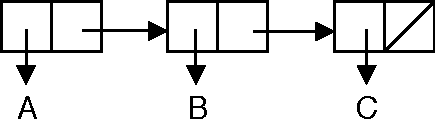
\includegraphics[width=4.2cm]{topics/bi-wsi-si-15/images/list}
  \caption{\mintinline{lisp}{(A B C)}}
\end{minipage}%
\begin{minipage}{.5\textwidth}
  \centering
  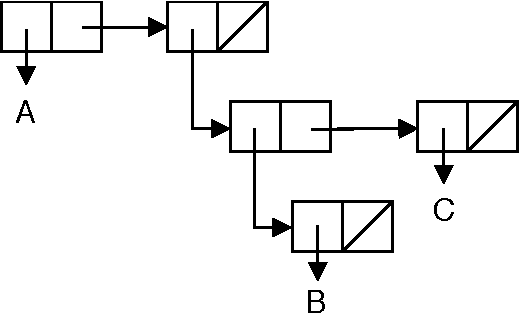
\includegraphics[width=4.8cm]{topics/bi-wsi-si-15/images/list-inner}
  \caption{\mintinline{lisp}{(A ((B) C))}}
\end{minipage}%
\end{figure}

\begin{figure}[H]
\centering
\begin{minipage}{.5\textwidth}
  \centering
  
\includegraphics[width=1cm]{topics/bi-wsi-si-15/images/list-empty}
  \caption{Prázdný seznam \mintinline{lisp}{() = NIL}}
\end{minipage}%
\begin{minipage}{.5\textwidth}
  \centering
  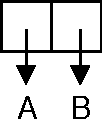
\includegraphics[width=1cm]{topics/bi-wsi-si-15/images/list-cons}
  \caption{\mintinline{lisp}{(A ((B) C))}}
\end{minipage}%
\end{figure}

\subsubsection*{Seznam}
\mintinline{lisp}{(cons 1 (cons 2 (cons 3 nil))) |$\Leftrightarrow$| (list 1 2 3)| je ve výsledku |(1 . (2 . (3 . nil)))}

\subsubsection*{Strom}
\mintinline{lisp}{(cons (cons 1 2) (cons 3 4))| je ve výsledku |((1 . 2) . (3 . 4))}

\subsubsection*{Výběr ze seznamu}
\begin{figure}[H]
  \centering
  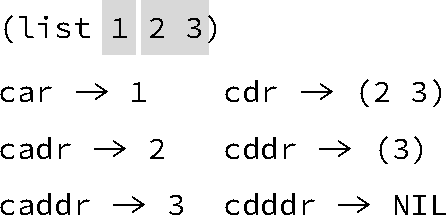
\includegraphics[width=4.2cm]{topics/bi-wsi-si-15/images/list-cdr}
  \caption{Ukázka výběru prvků ze seznamu}
\end{figure}

\subsection{Funkce}
\mintinline{lisp}{(defun name (parameters) (body))}

\begin{minted}{lisp}
(defun sum (x y) (+ x y))
(defun factorial (n) (if (zerop n) 1 (* n (factorial (- n 1)))))
\end{minted}

\subsection{Podmínky}
\begin{figure}[H]
\centering
\begin{minipage}{.5\textwidth}
  \centering
  \begin{minted}{lisp}
(defun abs (X)
 (cond ((> X 0) X) 
       ((= X 0) 0) 
       ((< X 0) (- X)) 
))
  \end{minted}
\end{minipage}%
\begin{minipage}{.5\textwidth}
  \begin{minted}{lisp}
(defun abs (X)
  (if (> X 0) X
   X
   (if (= X 0) 0 (- X))
))
  \end{minted}
\end{minipage}%
\end{figure}

\subsection{Rekurze}
Rekurze používá zasobník pro zachování stavu při vnoření do funkce (aktivační záznam). Doporučuje se využívat koncovou rekurzi, která šetří místo na zásobníku.

\begin{description}
\item[Vnořená] - rekurze v rekurzi
\item[Stromová] - několik rekurzivních volaní
\item[Lineární] - jedno rekurzivní volání
\item[Koncová] - rekurzivní volání je poslední, co funkce udělá - optimizace překladačů znovupoužití stejného stack framu
\end{description}


\begin{minted}{lisp}
(defun factorial (N)
  ;;;"Compute the factorial of N."
  (if (= N 0)
    1
    (* N (factorial (- N 1)))
))

(defun fast-factorial (N)
  ;;;"A tail-recursive version of factorial."
  (fast-factorial-aux N 1)
)

(defun fast-factorial-aux (N ACC)
  ;;;"Multiply A by the factorial of N."
  (if (= N 0)
    ACC
    (fast-factorial-aux (- N 1) (* N ACC))
))
\end{minted}


\subsection{Mapovací funkcionály}
Funkcionál je funkce, která má funkci jako argument.
  \mintinline{lisp}{(mapcar function list-1 list-2 ... list-n )}

Aplikujeme funkci square na list s položkami 1 2 3
  \mintinline{lisp}{(mapcar #'square '(1 2 3))}

\begin{itemize}
\item \mintinline{lisp}{mapcar} prochází všechny seznamy prvek po prvku. Ukončí se jakmile v některém z listů dojdou prvky. Návratovou hodnotou je list s prvky původních listů, na které byla aplikována funkce.
\item \mintinline{lisp}{mapc} funguje jako mapcar - vrací první list
\item \mintinline{lisp}{maplist} prochází list prvek po prvku, do další iterace jde vždy cdr ze zpracovaného listu
\end{itemize}

\begin{minted}{lisp}
(defun plus (x y) (+ x y))
(defun square (x) (* x x))

(mapcar #'square '(1 2 3)) |$\rightarrow$| (1 4 9)
(mapcar #'plus '(1 2 3) '(3 2 1)) |$\rightarrow$| (4 4 4)
(mapc #'plus '(1 2 3) '(3 2 1)) |$\rightarrow$| (1 2 3)
\end{minted}

\end{document}
